%%%%%%%%%%%%%%%%%%%%%%%%%%%%%%%%%%%%%%%%%%%%%%%%%%%%%%%%%%%%%%%%%%%%%%%%%%%%%%

\chapter{FUNDAMENTAÇÃO}\label{ch:fun}

Este capítulo apresenta os conceitos fundamentais relacionados a essa proposta, começando pela operação dos satélites na seção~\ref{ch:fun:operations}, apresentando a definição de \textit{Big Data} na seção~\ref{ch:fun:bigdata}, e os os conceito de \textit{Data Warehouse} na seção~\ref{ch:fun:dw}, \textit{OLAP} na seção~\ref{ch:fun:olap} e Cubo de Dados na seção~\ref{ch:fun:cube}.

\section{Operação de Satélites}\label{ch:fun:operations}

Um satélite é dividido em dois módulos: o módulo de serviço e a carga útil.
O módulo de serviço compõe tudo necessário para o funcionamento dos equipamentos de bordo, como o sistema de geração de energia, o sistema de comunicação com o solo, o computador de bordo, etc.
A carga útil compõe todos os equipamentos necessários para cumprir os objetivos da missão, sendo esses sensores, câmeras, telescópios, etc~\cite{larsonSpaceMissionAnalysis1999}.

Um satélite gera dois tipos diferentes de dados: dados da carga útil e dados de telemetria.
Os dados da carga útil são os dados gerados para cumprir a missão do satélite, sendo que eles podem ser fotos tiradas para o sensoriamento remoto, fotos tiradas por telescópios, dados de comunicação caso este seja o foco da missão entre outros~\cite{larsonSpaceMissionAnalysis1999}.
Os dados de telemetria são os dados de monitoramento do estado de saúde e do funcionamento dos equipamentos do satélite.
Esses dados são coletados pelo computador de bordo do satélite, e são enviados para as estações de solo via sistemas de telecomunicação.

Os dados de telemetria compõe usualmente medidas de sensores nos equipamentos do satélite, informações coletadas pelo computador de bordo (como se um instrumento está ligado ou não), e outros dados cuja coleta foi definida como relevante para a operação do satélite.
Dependendo da missão, outras medidas podem ser classificadas como telemetria, como por exemplo câmeras voltadas para o satélites, radares para a detecção de possíveis colisões, etc~\cite{kragCmSpaceDebris2017}.

Esses dados devem ser analisados pelos operadores de satélite em solo após recebimento no centro de controle.
Essa análise visa garantir que o satélite está executando suas tarefas como deveria, e que o seu estado de saúde permite a continuação da missão.
Neste trabalho, vamos utilizar da análise feita pelos operadores de satélite somente nos dados de telemetria.

\section{Big Data}\label{ch:fun:bigdata}

O termo \textit{Big Data} vem evoluindo ao longo dos anos, e para este trabalho vamos utilizar a definição dos \textit{5 Vs}~\cite{kacfahemaniUnderstandableBigData2015}: Volume, Variedade, Velocidade, Valor e Veracidade. Em detalhes:

\begin{itemize}
	\item \textbf{Volume}: esse termo geralmente especifica uma quantidade de dados em que um sistema tradicional de gerenciamento de banco de dados é ineficaz.
É importante ressaltar que isso não se trata apenas do armazenamento dos dados, mas também do seu processamento~\cite{boussoufBigDataBased2018}.
Usar um grande volume de dados geralmente implica em modelos melhores, que então produzem análises melhores, justificando a coleta de uma grande quantidade de dados.
	\item \textbf{Variedade}: dados são provenientes de fontes diferentes, com formatos diferentes, sem um esquema de modelagem padronizado, como dados advindos de \textit{logs} de computadores, dados de sensores, dados multimídia, etc.
Como consequência, esses dados devem ser utilizados da forma mais transparente o possível na análise.
	\item \textbf{Velocidade}: dados são disponibilizados de uma forma muito rápida, e devem ser analisados da forma mais rápida o possível.
Isso implica que os dados podem ser guardados e analisados até em tempo real.
	\item \textbf{Valor}: os dados devem ser armazenados para criar algum valor para os seus usuários, seja ele econômico, científico, social, organizacional, etc.
	\item \textbf{Veracidade}: os dados não possuem garantias quanto a sua qualidade, como inconsistências e falta de acurácia, porém a análise deve ser de alta qualidade de qualquer forma.
\end{itemize}

Estes V's estão relacionados com a construção de um \textit{Data Warehouse}, sendo que também podem ser vistos como requisitos para a crição de um para um conjunto de dados caracterizado como \textit{Big Data}~\cite{zhangBigDataFramework2017}.
Em especial, existe um certo relacionamento com a ideia de ``\textit{NoSQL}'' (``Não apenas SQL'', em inglês), em que não apenas sistemas de banco de dados relacionais são utilizados, mas também outros paradigmas são utilizados, como orientados a documentos, chave e valor, etc~\cite{bimonteOpenIssuesBig2016}.

\section{Data Warehouse}\label{ch:fun:dw}

Um Armazém de Dados ou Data Warehouse (DW) é um repositório de dados orientado por assunto, integrado, variado ou particionado em função do tempo e não volátil, que auxilia no gerenciamento do processo de tomada decisões~\cite{inmonUsingDataWarehouse1994}.
Essa definição pode ser dividida em:

\begin{itemize}
	\item \textbf{Orientado por assunto}: o DW é utilizado para a análise de uma área em específico.
Por exemplo, é de interesse analisar especialmente os dados da carga útil de uma forma específica.
	\item \textbf{Integrado}: o DW deve integrar dados vindos de múltiplas fontes de uma forma estrutura.
Por exemplo, mesmo que existam duas representações diferentes para um mesmo produto, o DW deve possuir apenas uma representação.
Isso requer o uso de técnicas de limpeza e integração dos dados, de modo a garantir a consistência dos dados.
	\item \textbf{Variado em função do tempo}: o DW deve conter, explícita ou implicitamente a perspectiva de tempo.
Isso quer dizer que o DW possui dados históricos e eles podem ser consultados durante a análise.
Por exemplo, pode se querer saber de dados de dias, meses ou anos atrás.
	\item \textbf{Não volátil}: uma vez dentro do DW, os dados não são removidos ou atualizados, sendo um requisito para a consulta de dados históricos.
\end{itemize}

Essas características diferem o \textit{Data Warehouse} de outros sistemas de repositório, como sistemas de banco de dados, sistemas de processamento de transações e sistemas de arquivos~\cite{hanDataMiningConcepts2011}.

Um DW é geralmente representado por um modelo dimensional que permite eficiência na organização dos dados e na recuperação de informações gerenciais~\cite{kimballDataWarehouseToolkit2013}.
Neste modelo são definidos fatos, dimensões e medidas.
Um fato corresponde ao assunto de negócio a ser analisado, cada dimensão é uma perspectiva de visualização do assunto de negócio e medidas são valores numéricos que quantificam o assunto de negócio.
Uma das dimensões é sempre temporal para permitir a análise do assunto ao longo do tempo~\cite{silva:2015:abordagensParaCubo}.

\section{OLAP}\label{ch:fun:olap}

\textit{On-line Analytical Processing} (OLAP) é um termo que se refere a um conjunto de ferramentas que são utilizadas para resumir, consolidar, visualizar, aplicar formulações e sintetizar dados de acordo com múltiplas dimensões~\cite{coddProvidingOlapUseranalysts1998}.

Um sistema OLAP permite a resposta de consultas multidimensionais usando dados armazenados no \textit{Data Warehouse}~\cite{kimballDataWarehouseToolkit2013}, sendo que as características principais são~\cite{bimonteOpenIssuesBig2016}:

\begin{itemize}
	\item \textbf{Consultas Online}: as consultas devem ser feitas \textit{Online}, isto é, em tempo real para o usuário.
	\item \textbf{Consultas Multidimensionais}: Consultas são definidas utilizando as dimensões e medidas providas pelo \textit{Data Warehouse}, que esperam dados de alta qualidade.
	\item \textbf{Representação simples}: os resultados das consultas devem ser representados utilizando tabelas e gráficos, pois os usuários finais geralmente são tomadores de decisão que precisam de visualizações relevantes.
	\item \textbf{Exploratórias}: as consultas são utilizadas em carácter exploratório, pois geralmente os usuários não conhecem de antemão todos os dados disponíveis para consultas.
\end{itemize}

Cada ferramenta OLAP deve manipular um novo tipo abstrato de dados (TAD), chamado de cubo de dados, utilizando estratégias específicas devido ao modo de como os dados são armazenados, sendo classificadas em~\cite{moreiraFullPartialData2012}:

\begin{itemize}
	\item \textbf{\textit{Relational OLAP} (ROLAP)}: utilizam Sistemas de Gerenciamento de Banco de Dados (\textit{Data base Management System} - DBMS) relacionais para o gerenciamento e armazenamento dos cubos de dados.
Ferramentas ROLAP incluem otimizações para cada DBMS, implementação da lógica de navegação em agregações, serviços e ferramentas adicionais;
	\item \textbf{\textit{Multidimensional} OLAP (MOLAP)}: implementam estruturas de dados multidimensionais para armazenar cubo de dados em memória principal ou em memória externa.
Não há utilização de repositórios relacionais para armazenar dados multidimensionais e a lógica de navegação já é integrada a estrutura proposta;
	\item \textbf{\textit{Hybrid} OLAP (HOLAP)}: combinam técnicas ROLAP e MOLAP, onde normalmente os dados detalhados são armazenados em base de dados relacionais (ROLAP), e as agregações são armazenadas em estruturas de dados multidimensionais (MOLAP).
\end{itemize}

Além desses, existem sistemas OLAP voltados para um domínio ou estilo de dados específico, como é o caso do \textit{Spatial OLAP} (SOLAP), voltado para consultas espaciais~\cite{viswanathanUsercentricSpatialData2014}.

É importante ressaltar a diferença entre OLAP e \textit{Online Transaction Processing} (OLPT), visto que sistemas comuns de banco de dados utilizam apenas OLTP, que tem o objetivo de realizar transações e processar consultas online.
Isso cobre a grande maioria das operações do dia a dia, como controle de estoque, operações bancárias, etc, servindo a diversos usuários de uma organização.
Já o OLAP é utilizado por tomadores de decisão e analistas de dados, sendo voltado para decisões de mais alto nível na organização~\cite{hanDataMiningConcepts2011}.

\section{Cubo de Dados}\label{ch:fun:cube}

O Cubo de Dados originalmente foi criado como um operador relacional que gera todas as combinações possíveis de seus atributos de acordo com uma medida~\cite{grayDataCubeRelational1996}.

A estrutura do cubo de dados permite que os dados sejam modelados e visualizados em múltiplas dimensões, e ele é caracterizado por dimensões e medidas.
Uma medida é um atributo cujos valores são calculados pelo relacionamento entre as dimensões, sendo que esse é calculado utilizando funções de agragação como soma, quantidade, média, moda, mediana, etc.
Uma dimensão é feita pelas entidades que compõe os nossos dados, determinando o contexto do assunto em questão~\cite{hanDataMiningConcepts2011}.
Uma dimensão pode ainda ser dividida em membros, que podem ter uma hierarquia, como uma divisão da dimensão tempo em dia, mês e ano.

A organização de um cubo de dados possibilita ao usuário a flexibilidade de visualização dos dados a partir de diferentes perspectivas, já que o operador gera combinações através do conceito do valor \textit{ALL}, onde este conceito representa a agregação de todas as combinações possíveis de um conjunto de valores de atributos.
Operações em cubos de dados existem a fim de materializar estas diferentes visões, permitindo busca e análise interativa dos dados armazenados~\cite{hanDataMiningConcepts2011}.

Um cubo de dados é composto por células e cada célula possui valores para cada dimensão, incluindo \textit{ALL}, e valores para as medidas.
O valor de uma medida é computado para uma determinada célula utilizando níveis de agregação inferiores para gerar os valores dos níveis de agregação superiores na estratégia \textit{Top-down}, com a ordem inversa sendo a \textit{Bottom-up}.

\begin{figure}[!htb]
	\caption{Exemplo de um cubo de dados \color{red}Substituir pelo exemplo do rodrigo}\label{fig:cubeexample}
	\vspace{2mm}
	\begin{center}
		\resizebox{9cm}{!}{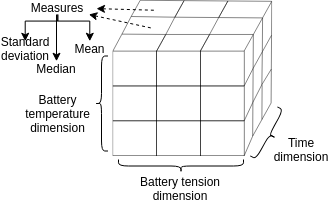
\includegraphics{Figuras/DataCube-Fig1.png}}
	\end{center}
	\vspace{1mm}
	\legenda{}
	\FONTE{Produção do autor}.
\end{figure}

\subsection{Células do Cubo de Dados}\label{ch:fun:cube:cells}

{\color{red} Lattice}

Um cubo de dados é composto de vários subcubos, que são todos os possíveis níveis de agregação nas dimensões especificadas.
Subcubos são compostos de células base e células agregadas, sendo uma célular agregada é uma célula que utiliza do valor especial \textit{ALL} (``$*$'') para demonstrar que está agregando valores em uma ou mais dimensões.
Uma célula base não utiliza da notação \textit{ALL}, sendo composta do nível mais baixo de agregação~\cite{limaSEQUENTIALPARALLELAPPROACHES2009}.

Formalmente, supondo um cubo de dados $n$-dimensional, uma célula $a$ de qualquer subcubo é definida por $a = (a_1, a_2, a_3, \ldots, a_n, medidas)$.
A célula é m-dimensional (de um subcubo com $m$ dimensões), se exatamente $m$, com $(m \leq n)$, valores entre $(a_1, a_2, a_3, \ldots, a_n)$ não são ``$*$''.
Se $m = n$, então $a$ é uma célula base, caso contrário $(m < n)$, ela é uma célula agregada.

{\color{red} exemplo?}

Um relacionamento de descendente-ancestral pode existir entre células.
Em um cubo de dados $n$-dimensional, uma célula $a = (a_1, a_2, a_3, \ldots, a_n, medidas_a)$ de nível $i$ é um ancestral de uma célula $b = (b_1, b_2, b_3, \ldots, b_n, medidbs_b)$ de nível $j$, e $b$ é um descendente de $a$, se e somente se $i < j$ e $1 \leq m \leq n$, onde $a_m = b_m$ sempre que $a_m \neq *$.
Em particular, uma célula $a$ é chamada de pai de uma célula $b$, e $b$ de filho de $a$, se e somente se $j = i+1$ e $b$ for um descendente de $a$~\cite{hanDataMiningConcepts2011}.

{\color{red} exemplo}

\subsection{Modelagem dimensional}\label{ch:fun:cube:dimm}

Existem três esquemas principais para a modelagem dimensional de um cubo de dados: Esquema Estrela (\textit{Star Schema}), Esquema Floco de Neve (\textit{Snowflake Schema}) e Constelação de Fatos (\textit{Fact Constellation Schema}).

O esquema estrela é o mais utilizado, sendo que ele contém uma tabela central chamada de tabela de fatos, onde reside a maior parte dos dados, com um conjunto menor de tabelas, chamadas de tabelas de dimensão, para as outras dimensões.
A figura~\ref{fig:starschema} mostra um exemplo de esquema estrela.

\begin{figure}[!htb]
	\caption{Esquema estrela}\label{fig:starschema}
	\vspace{6mm}
	\begin{center}
		\resizebox{4cm}{!}{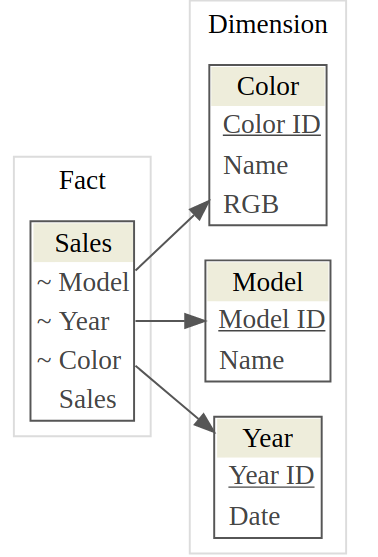
\includegraphics{Figuras/starSchema.png}}
	\end{center}
	\vspace{1mm}
	\legenda{}
	\FONTE{Produção do autor}.
\end{figure}

O esquema floco de neve é uma variação do esquema estrela, onde algumas dimensões são normalizadas, dividindo os dados das tabelas de dimensão em outras tabelas.
Isso possui vantagens de eliminar redundâncias nas tabelas de dimensão, porém cria problemas durante a execução de consultas, visto que é necessário realizar operações de \textit{join} com as novas tabelas.
A figura~\ref{fig:snowflakeschema} mostra um exemplo de esquema floco de neve.

\begin{figure}[!htb]
	\caption{Esquema floco de neve}\label{fig:snowflakeschema}
	\vspace{2mm}
	\begin{center}
		\resizebox{5cm}{!}{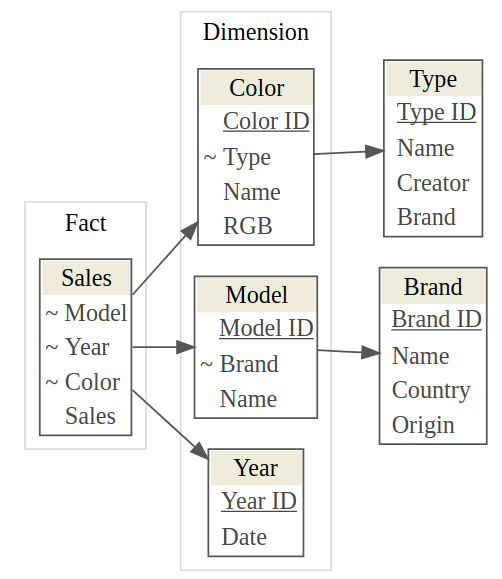
\includegraphics{Figuras/snowflakeSchema.png}}
	\end{center}
	\vspace{1mm}
	\legenda{}
	\FONTE{Produção do autor}.
\end{figure}

O esquema constelação de fatos utiliza de múltiplas tabelas de fato, como se fossem várias tabelas no esquema estrela que compartilham tabelas de dimensão.
Isso leva ao seu nome, como um conjunto de estrelas.
A figura~\ref{fig:factconstschema} mostra um exemplo de constelação de fatos.

\begin{figure}[!htb]
	\caption{Esquema constelação de fatos}\label{fig:factconstschema}
	\vspace{6mm}
	\begin{center}
		\resizebox{7cm}{!}{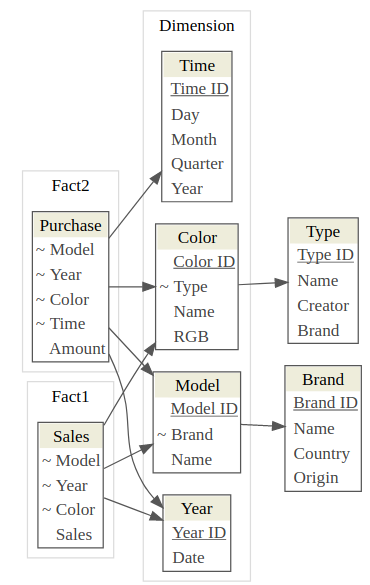
\includegraphics{Figuras/factConstellationSchema.png}}
	\end{center}
	\vspace{2mm}
	\legenda{}
	\FONTE{Produção do autor}.
\end{figure}

\subsection{Hierarquias de conceito}\label{ch:fun:cube:concept}

Uma hierarquia de conceitos é utilizada para definir uma sequência de mapeamento entre um conjunto de conceitos de baixo nível para um conjunto de conceitos de alto nível, mais gerais.
É um estilo de agrupamento e discretização, pois agrupa os valores de modo a reduzir a cardinalidade de uma dimensão~\cite{hanDataMiningConcepts2011}.
Elas ajudam a tornar a análise mais fácil de ser entendida, pois as operações traduzem os dados de baixo nível em uma representação que é mais fácil para o usuário final, assim facilitando a execução das consultas e o seu subsequente uso.

{\color{red} Han, figura 4.10}

\subsection{Medidas}\label{ch:fun:cube:measures}

Cada célula de um cubo é definida como um par $\langle (d_1, d_2, \ldots, d_n), medidas\rangle$, onde $(d_1, d_2, \ldots, d_n)$ representam as combinações possíveis de valores de atributos sobre as dimensões.
Uma medida é calculada para uma certa célula agregando os dados correspondentes a combinação de dimensões e valores~\cite{hanDataMiningConcepts2011}.
Medidas podem ser classificadas em três tipos: distributiva, algébrica e holística.

Uma medida distributiva é uma medida cujo cálculo pode ser particionado e depois combinado, e o resultado seria o mesmo se o cálculo fosse executado em todo o conjunto de dados.
Por exemplo, a função de soma é distributiva: dividindo os dados $N$ em conjuntos $n$, e fazendo a soma de cada conjunto $n$, teremos o mesmo resultado que se a fosse feita diretamente sobre $N$.

Uma medida algébrica é uma medida cujo cálculo pode ser feito sobre duas ou mais medidas distributivas.
Por exemplo, uma medida de média pode ser calculada com a divisão da medida \textit{soma} pela a medida \textit{contagem}, que são ambas distributivas.

Uma medida é holística se não existe uma medida algébrica com $M$ argumentos que caracterize a computação.
Isso quer dizer que a computação não pode ser particionada, com valores exatos obtidos apenas se a medida for aplicada em todos os dados.
Alguns exemplos são as medidas de moda, desvio padrão e mediana~\cite{hanDataMiningConcepts2011}.

\subsection{Operações OLAP}\label{ch:fun:cube:olapops}

Para realizar consultas no \textit{Data Warehouse}, é necessário utilizar de algumas operações sobre o cubo de dados para obter os resultados adequados.
Essas consultas também devem conseguir passar na hierarquia de conceitos de cada dimensão, bem como seguir o modelo dimensional do cubo definido, para conseguir oferecer uma interface amigável com o usuário para análise interativa~\cite{hanDataMiningConcepts2011}.
Algumas operações comuns são:

\begin{itemize}
	\item \textit{Roll-up}: realiza agregação no cubo de dados, seja navegando na hierarquia de conceitos de nível específico para um mais genérico, ou reduzindo uma dimensão.
	\item \textit{Drill-down}: o inverso da operação \textit{roll-up}, navega na hierarquia de conceitos do nível mais genérico para o nível mais específico, ou adiciona dimensões ao cubo atual.
Essa operação visa aumentar o nível de detalhes dos dados.
	\item \textit{Slice}: ou ``fatiamento'', realiza uma seleção em uma dimensão do cubo, resultando em um subcubo.
	\item \textit{Dice}: define um subcubo realizando uma seleção (\textit{slice}) em duas ou mais dimensões.
	\item \textit{Pivot}: também chamada de rotação, permite mudar a posição das dimensões na visualização, portanto alterando linhas por colunas e vice-versa.
\end{itemize}

{\color{red} Rodrigo, figura 2.1}

Dependendo do sistema OLAP, é possível que outras operações sejam possíveis, como \textit{drill-across} que passa por mais do que uma tabela de fatos, e \textit{drill-through} que permite executar consultas direto na representação em baixo nível do cubo~\cite{hanDataMiningConcepts2011}.

\subsection{Computação do cubo de dados}\label{ch:fun:cube:comp}

{\color{red} Qual a definição de uma tarefa ``essencial''?}

A computação do cubo de dados é uma tarefa {\color{red} essencial}, pois a pré-computação de todo ou parte de um cubo de dados pode aumentar significativamente o desempenho do DW.
Porém, essa tarefa possui complexidade exponencial em relação ao número de dimensões, sendo chamada de materialização, com a materialização completa exigindo uma grande quantidade de células, e portanto um elevado consumo de memória e tempo~\cite{hanDataMiningConcepts2011}.

O cálculo original da computação do cubo de dados foi proposta por~\cite{grayDataCubeRelational1996}, sendo: dada uma relação de relação de entrada $R$ com tuplas de tamanho $n$, o número de subcubos que podem ser gerados é $2^n$, onde $n$ é o número de dimensões do cubo.
Por exemplo, supondo um cubo com três dimensões \textit{Satélite, Telemetria, Valor}, teremos $2^3 = 8$ subcubos possíveis: $\{(satélite, telemetria, valor), (satélite, valor), (satélite, telemetria),$ $(telemetria, valor), (telemetria), (valor), (satélite), () \}$, com $()$ denotando o agrupamento vazio (célula base, as dimensões não estão agrupadas).
% Weird latex thing here...

Porém, na prática, as dimensões podem possuir hierarquias de conceito associadas, como para a dimensão tempo: ``dia<mês<trimestre<semestre<ano''.
Para um cubo com $n$ dimensões com múltiplas hierarquias de conceito, o número total de subcubos é apresentado na equação~\ref{eq:conceptcuboids}.

\begin{equation}
	subcubos = \prod_{i=1}^n (L_i + 1)
\label{eq:conceptcuboids}
\end{equation}

Onde $L_i$ é o número de níveis de conceito da dimensão $i$.
É necessário adicionar um a equação~\ref{eq:conceptcuboids} para denotar o nível virtual \textit{ALL}.
O tamanho de cada subcubo também depende da cardinalidade de cada dimensão, isto é, o número de valores distintos.
Enquanto o número de dimensões, hierarquias de conceito e cardinalidade do cubo aumenta, também aumentam os seus requisitos de espaço de forma exponencial, sendo conhecida como a \textbf{maldição de dimensionalidade} na computação do cubo~\cite{hanDataMiningConcepts2011}.

Para conseguir responder as consultas de maneira apropriada, é necessário escolher um método para a computação dos subcubos: a não materialização, a materialização completa e a materialização parcial.

Na não materialização, os subcubos agregados não são pré-computados, assim as agregações são computadas imediatamente, que podem ser extremamente lentas, porém tem o menor consumo de memória.

A materialização completa computa todos as agregações possíveis do cubo, gerando um cubo de dados completo.
Esse método gera os melhores tempos de resposta, pois as agregações já foram computadas, porém necessita de uma grande quantidade de espaço de memória.

A materialização parcial computa apenas um subconjunto selecionado de subcubos, sendo que existem diversas técnicas diferentes de seleção dos subcubos que serão computados.
Uma delas é computar todos os subcubos que contém apenas células que satisfazem um dado critério, especificado pelo usuário.
Esses cubos são chamados de \textit{iceberg}~\cite{beyerBottomupComputationSparse1999}.

Outra técnica é computar cubos pequenos, geralmente entre 3 e 5 dimensões, para formar cubos completos.
Para responder consultas com mais dimensões, as combinações entre os subcubos pequenos são agregadas.
Esta técnica é chamada de \textit{shell fragment}, e o cubo é chamado de \textit{cube shell}~\cite{liHighdimensionalOLAPMinimal2004}.

Um cubo de dados onde as células com medidas idênticas são encapsuladas em uma única abstração, chamada de célular fechada (\textit{closed cell}) é chamado de cubo fechado, ou cubo quociente.
Esta técnica foi apresentada com o cubo fechado (\textit{closed cube})~\cite{dongxinCCubingEfficientComputation2006} e com o cubo quociente (\textit{quotient cube})~\cite{lakshmananQuotientCubeHow2002}.

A escolha da materialização parcial depende do equilíbrio necessário entre tempo de resposta e espaço de armazenamento.
Porém, a computação do cubo completo continua sendo relevante, sendo que os avanços na computação dos cubos parciais são geralmente adotados na computação do cubo completo.
Existe ainda o problema de atualização do cubo, pois cada atualização pode causar uma recomputação parcial ou completa do cubo para manter as medidas corretas.

A partir de um cubo base, a computação do cubo de dados pode utilizar a estratégia \textit{Top-down} ou \textit{Bottom-up} para a geração dos subcubos remanescentes~\cite{hanDataMiningConcepts2011}.

A figura~\ref{fig:topdown} mostra a geração de um cubo de dados de quatro dimensões pela estratégia \textit{Top-down}.
Sendo ABCD um cubo base, os subcubos de três dimensões são: ABC, ABD, ACD e BCD; que podem utilizar os resultados do cubo base para serem computados.
Os resultados da computação do subcubo ACD pode ser utilizado para computar AD, que consequentemente pode ser utilizado para computar A.
Essa computação compartilhada permite que a estratégia \textit{Top-down} compute agregações em múltiplas dimensões.
Os valores agregados intermediários podem ser reutilizados para a computação de subcubos descendentes sucessivos.

\begin{figure}[!htb]
	\caption{Computação de cubo de dados através da estratégia \textit{Top-Down}}\label{fig:topdown}
	\vspace{4mm}
	\begin{center}
		\resizebox{8cm}{!}{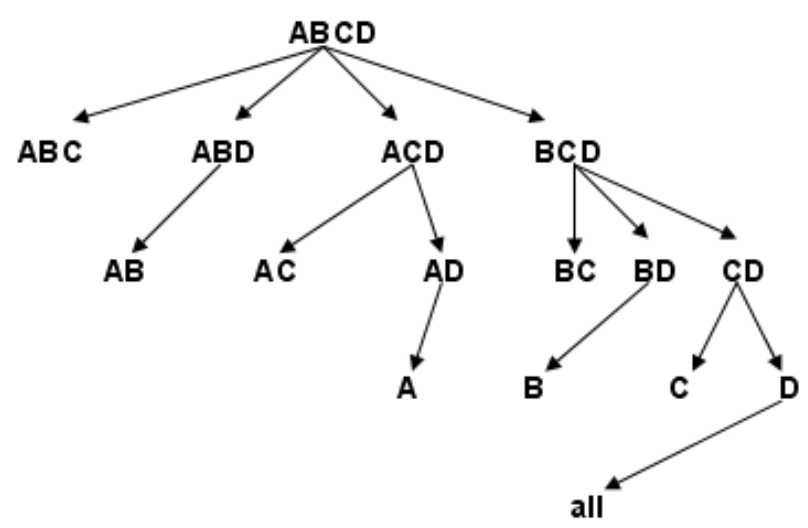
\includegraphics{Figuras/topdown.png}}
	\end{center}
	\vspace{2mm}
	\legenda{}
	\FONTE{~\cite{silva:2015:abordagensParaCubo}}.
\end{figure}

Na Figura~\ref{fig:bottomup}, é ilustrada a geração de um cubo de dados de 4 dimensões por meio da estratégia \textit{Bottom-up}.
Subcubos de poucas dimensões tornam-se pais de subcubos com mais dimensões.
Infelizmente, a computação compartilhada, utilizada na estratégia \textit{Top-down}, não pode ser aplicada quando utilizada a estratégia \textit{Bottom-up}, então cada subcubo descendente necessita ser computado do início.

\begin{figure}[!htb]
	\caption{Computação de cubo de dados através da estratégia \textit{Bottom-up}}\label{fig:bottomup}
	\vspace{4mm}
	\begin{center}
		\resizebox{8cm}{!}{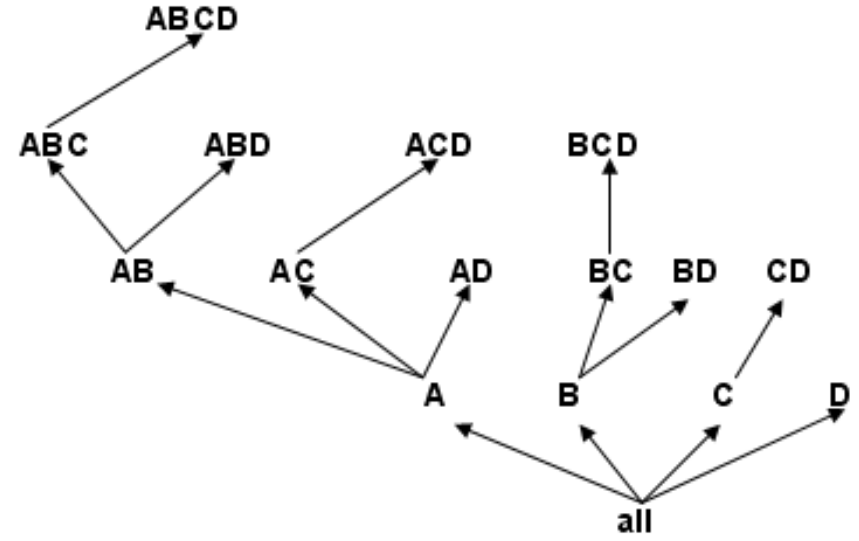
\includegraphics{Figuras/bottomup.png}}
	\end{center}
	\vspace{2mm}
	\legenda{}
	\FONTE{~\cite{silva:2015:abordagensParaCubo}}.
\end{figure}

